From the discovery of the \gls{dna} structure by Watson and Crick in
1953\cite{watson1953molecular} to the sequencing of the human genome in 2001
\cite{venter2001sequence,international2001initial} and the massively parallel
sequencing platforms in the later years[6], the scientific advances have been
tremendous. Today, single week-long sequencing runs can produce as much data as
did entire genome centers just years ago.\cite{kahn2011future}  These
technologies allow researchers to produce data faster, cheaper and more
efficiently, now making it possible to sequence the entire genome from a patient in
less than a days work.

In this chapter we give a background in the different aspects of analyzing and
exploring biological datasets. We use the \gls{nowac} study as an example and
highlight the necessary processing steps from data generation and to
interpretation of results. In addition we describe the traditional data analysis
and management, and propose a novel approach for organizing, sharing, and
collaborating on research data and analyses. In this chapter we focus on
analysts in the \gls{nowac} study writing their own specialized analysis scripts
in the R programming language.

\section{High-Throughput Datasets for Research and Clinical Use} 
Cells are the smallest units an organism can be divided into, that still
possesses the functions performed by living organisms. Within cells we find
proteins, the working units, found in a wide range of processes.  All cells
within an organism contain the same genetic information, this genetic
information is stored within nucleic acids which are responsible for storage,
transmission and expression. There are two types of nucleic acids, \gls{dna} and
\gls{rna}.  DNA is responsible for the storage of genetic information, while RNA
is used in decoding the information stored within DNA. Genes are sequences of
\gls{dna}, and the human genome consists of approximately 20 500 genes. These
genes specify how proteins are synthesized. In short, DNA is transcribed into
RNA which are translated to proteins. This is called the central dogma of
molecular biology. 

\gls{dna} sequencing is the process of determining the order of nucleotides
within a strand of \gls{dna}. \gls{hts}, or \gls{ngs}, is a term used to
described newer technology that enables massively-parallel sequencing of
\gls{dna}. \gls{hts} instruments sequence millions of short base pairs and
we assemble these in the data analysis process. Typical sequencing datasets are
in the size of hundreds of \glspl{gb} per sample. 

While \gls{hts} can study the sequence of bases, we use \gls{dna} microarrays to
study the transcriptome, or the genes actively expressed. While the genome is
mostly fixed for an organism, the transcriptome is continuously changing. These
instruments report the expression levels of a large number of target genes, and
by profiling these we can study which genes are active in the biological sample.
Microarray datasets are in the size of of megabytes per sample. 

Another technique to study the transcriptome is to use \gls{rna}-seq technology
based on \gls{hts}. \gls{rna}-seq instruments also read millions of short base
pairs in parallel, and can be used in gene expression analysis. Because of its
higher quality output, \gls{rna}-seq is the successor to microarray technology.
These datasets are also in the size of hundreds of \glspl{gb}.

Precision medicine uses patient-specific molecular information to diagnose and
categorize disease to tailor treatment to improve health
outcome.\cite{national2011toward} Important research goal in precision medicine
are to learn about the variability of the molecular characteristics of
individual tumors, their relationship to outcome, and to improve diagnosis and
therapy.\cite{tannock2016limits} International cancer institutions are therefore
offering dedicated personalized medicine programs, but while the data collection
and analysis technology is emerging, there are still unsolved problems to enable
reproducible analyses in clinical settings. For cancer, \gls{hts}
is the main technology to facilitate personalized diagnosis and
treatment since it enables collecting high quality genomic data from patients
at a low cost. 

\section{Norwegian Women and Cancer (\gls{nowac})} 
The \gls{nowac} study is a prospective population-based cohort that tracks 34\%
of all Norwegian women born between 1943–57.\cite{lund2007cohort} We started the
data collection in \gls{nowac} in 1991 with questionnaires to cover, among
others, the use of oral contraceptives and hormonal replacement therapy,
reproductive history, smoking, physical activity, breast cancer, and breast
cancer in the family.  We also integrate the Norwegian Cancer Registry, the
register of the National Mammographic Screening Program, and the register of
death certificates in Statistics Norway.  In addition to the questionnaire data,
the \gls{nowac} biobank now contain blood samples from 50 000 women, as well as
tumor tissue samples. From the biological samples we have generated gene
expression, miRNA, methylation, and RNA sequencing datasets. 

From the \gls{nowac} cohort we have have published a number of research papers
that investigate the questionnaire data\cite{find-some-papers}. We have also
used the gene expression datasets to explore ... and interactions between the
tumor and the blood systemic response of breast cancer
patients.\cite{dumeaux2017interactions} While we have studied interesting
patterns and questions, there are still unexplored areas in the available
datasets.

\subsection{Data Management} 
In the \gls{nowac} study questionnaire data is stored on an in-house dedicated
database backed up to an independent storage node. The database is maintained by
a handful of personnel which are also responsible for extracting data for
researchers and projects. This is typically done through SAS scripts that
selects the applicable variables and samples, and optionally generate computed
variables such as smoking status from the questionnaire data. There is no
systematic version control of the datasets or processing scripts. 

In addition to the questionnaire data, the \gls{nowac} study also integrates
with registries which are updated regularly. The datasets from the different
registries are typically delivered as \gls{csv} files which are then processed
into a standardized format. Since the \gls{nowac} study is a prospective cohort
women are expected to get cancer and move from the list of controls into the
list of cases. 

In the \gls{nowac} study we have used third-party sources to process and analyze
biological samples. The resulting datasets were then stored on a local
compute-node and made available to researchers on demand. Because of the nature
of the biological datasets, many of these require extensive pre-processing
before they are analysis-ready. 

There are multiple drawbacks to managing the research datasets using the
traditional approach detailed above. First, it is a difficult task to retrace
original data when the data extraction scripts are not versioned and kept track
of in a shared repository. Second, while datasets are backed up, there is no
information about changes between dataset versions. For example, samples may be
removed and there is no record of these changes. 

\subsection{Data Analysis} 
Traditionally, researchers had to send an application to get data exported from
the database by an engineer. The downstream analysis of questionnaire data was
typically done in SAS on local computers.  Traditionally researchers have used
e-mail to communicate and share data analysis scripts, and there has not been a
central hub to share scripts or data. Because of the many packages in
Bioconductor\footnote{bioconductor.org} we have used R to analyse the different
gene expression datasets in the projcet. However like with SAS the researchers
have typically shared scripts through e-mail and there has not been a tradition
to version control the analysis scripts. Results from the analyses are often
communicated through research papers subsequently. 

There are several drawbacks to this approach. First, there are obvious drawbacks
of not version controlling analysis scripts 
Second, sharing analysis scripts through e-mail and not centralized repositories
makes it difficult to share code especially in research groups with researcher
turnover. 
Third, using proprietary software
such as SAS makes it difficult for anyone without the necessary licences to
revisit the analyses. Last, separating the reporting of the results from the
actual data analysis leaves room for human errors when generating tables or
plots. 



\subsection{Requirement Analysis} 
To enable more researchers to benefit from the unique datasets in \gls{nowac} we
wanted to improve the way researchers access data as well as how they share
their analyses. By improving access and how the researchers share analyses we
are indirectly improving reproducibility in the project. 

Before developing an approach to standardize data management and analysis in the
\gls{nowac} study we performed a requirement analysis and determined the
following requirements for such systems: 

\begin{itemize} 
    \item It provides a single location for storing datasets and analysis code.
    \item it provides documentation for the datasets, how they are processed,
    and other useful information for downstream analyses. 
    \item It enables the standardization of pre-processing steps required to
    analyze biological datasets. 
\end{itemize}

From these requirements we designed and implemented i) a software package in the
R programming language that contain all datasets, their documentation, and
useful analysis functions to work with the data, and ii) a \gls{gui} for
to perform the necessary pre-processing steps before delivering
datasets to researchers, and iii) 
best practices for researchers that want to work with datasets from the
\gls{nowac} cohort. 
In the next sections we describe the software packages and best practices. 


\section{Modernizing Data Management and Analysis} 
The first step in modernizing the data management and analysis in the
\gls{nowac} study was to identify the possible environments to develop our
approach. While the majority of the researchers that have worked on the project
have used SAS for their analyses of the questionnaire data, all researchers
working on biological data are using R. Because of the number of additional
software  packages, its open-source implantation, and growing developer
community we have opted to implement our approach for managing and processing to
fit the R programming language. 

The great strength of R comes from its many packages for analyzing, plotting,
and interpreting data. An R package consists of a code, documentation, tests,
and data. Bioconductor and CRAN provide online hosing for a large number of
packages, and users can mix and match these packages to fit their need. 

We designed the \gls{nowac} R package to provide a single-stop location for
documentation, data, and analysis code for researchers within our research
group. We share this package within our group both as a repository that
researchers can contribute to, and a binary installer for basic uses. 
We use \texttt{git} to version control the analysis code and datasets, and store
the repository on a self-hosted git server (gitlab\footnote{\url{gitlab.com}}).
With git we can track changes to our analysis code, documentation, and datsets
over time. 

\subsection{Data management} 
We bundle together all datasets with the \gls{nowac} package. This includes both
questionnaire, registry, and biological datasets. Since none of these are
perticularly large in size (no single dataset being more than tens of
\glspl{gb}) we are able to distribute them with the software package. Some of
the datasets require pre-processing steps such as outlier removal before the
analysts can explore the datasets. For these datasets we store both the
\emph{raw} datasets as well as the analysis-ready clean datasets. We store the
raw datasets in their original format, while clean datasets are stored as R data
files to simplify importing them in R. In addition to the datasets themselves we
store the R code we used to generate the datasets. For clearity we decorate the
scripts with specially formatted comments that can be used with
knitr\footnote{\url{yihui.name/knitr}} to generate PDF reports. These highlight
the transformation of the data from raw to clean, with information such as
removed samples or data normalization methods. 

We document both code and each dataset with
roxygen2\footnote{\url{cran.r-project.org/web/packages/roxygen2}}. The
documentation is written as specially formatted comments to R source code and
allows us to special details such as data collection date, instrument types, the
persons involved with data collection and analysis, pre-processing methods etc.
When users install the \gls{nowac} package these comments are used to generate
interactive help pages which they can browse in R, be it the CLI or through
RStudio. 

As mentioned we use git to version control our \gls{nowac} package. There are
however drawbacks to creating one large repository for both data and code. Since
git stores every version of a file, these types of repositories may become large
if the datasets are changing a lot over time, and are stored in binary formats,
e.g. gene expression datasets. We have explored different techniques to minimize
our repository and have opted to store all datasets as git
submodules\footnote{\url{git-scm.com/docs/git-submodule}}. Submodules allow us
to keep the main repository size down while still versioning the data. Other
alternatives such as git-raw\footnote{\url{github.com/atofigh/git-raw}},
git-annex\footnote{\url{git-annex.branchable.com}} 
git-lfs\footnote{\url{git-lfs.github.com}} exist, and these all provide
alternative approaches to storing large binary files in the repository. We have
not found that any of these could satisfy our needs, mainly because they all
require a newer software stack than we have access to.

\subsection{Data processing} 
In the \gls{nowac} package we provide utility functions to get started with the
analysis of our datasets. Because of the specialized nature of the different
research project the \gls{nowac} package only contains helper functions to start
analyzing \gls{nowac} data, e.g. retrieving questionnaire data. 

\subsection{Best Practices} 
From our experiences we have developed a set of best practices for researchers
working on data analysis in the \gls{nowac} study. We believe that we can
generalize these to researchers working in different disciplines. 

\textbf{Document every step in the analysis}. Analysis of modern datasets is a
complex exercise with the possibility of introducing an error in every step.
Analysts often use different tools and systems that require a particular set of
input parameters to produce results. Thoroughly document every step from raw
data to the final tables that go into a manuscript.

In the \gls{nowac} study we write help pages and reports for all datasets, and
the optional pre-processing steps. 

\textbf{Generate reports and papers using code}. With tools such as R
Markdown\footnote{\url{rmarkdown.rstudio.com}}
and kntir there are few reasons for decoupling analysis code with the
presentation of the results through reports or scientific papers. Doing so
ensures the correctnes reported results from the analyses, and greatly
simplifies reproducing the results in a scientific paper. 

In the \gls{nowac} study we produce reports from R code. These include
pre-processing and data delivery of datasets to researchers. One example of a
report is the analyses done in \cite{kiselev2018transcription} where we
documented the association between PAX6 gene expression and PAX6 target genes.

\textbf{Version control everything}. Both code and data changes over the course
of a research project. Version control everything to make it possible to retrace
changes and the person responsible for them. It is often necessary to roll back
to previous versions or a dataset or analysis code, or to identify the
researches that worked on specific analyses. 

In the \gls{nowac} study we promote the use of git to version control both
source code and data. 

\textbf{Collaborate and share code through \gls{scm} systems}. Traditional
communication through e-mail makes it difficult to keep track of existing
analyses and their design choices both for existing project members and new
researchers. With \gls{scm} hosting systems such as Github developing
analysis code becomes more transparent to other collaborators, and encourages
collaboration. It also simplifies the process or archiving development decisions
such as choosing a normalization method.

In the \gls{nowac} study we collaborate on data analysis through a self-hosted
Gitlab\footnote{\url{gitlab.com}} installation. We also open-source our code on
Github. 


%\subsection{Discussion} 
% large datasets, e.g. sequencing 

\section{Pippeline}
The Pippeline is our approach to standardize the pre-processing and generation
of analysis-ready datasets in the \gls{nowac} study. It is a point-and-click
application that can be used by users without any prior programming experience.
The Pippeline application builds upon the \gls{nowac} R package, both
fundamentally but also through its design choices. It is targeted towards
researchers who want to start analyzing different datasets from the \gls{nowac}
cohort, and provides an automated system for performing the first steps of such
analyzes. 
Figure \ref{fig:scr_filtering} shows a screenshot of the web application.

\begin{figure}
  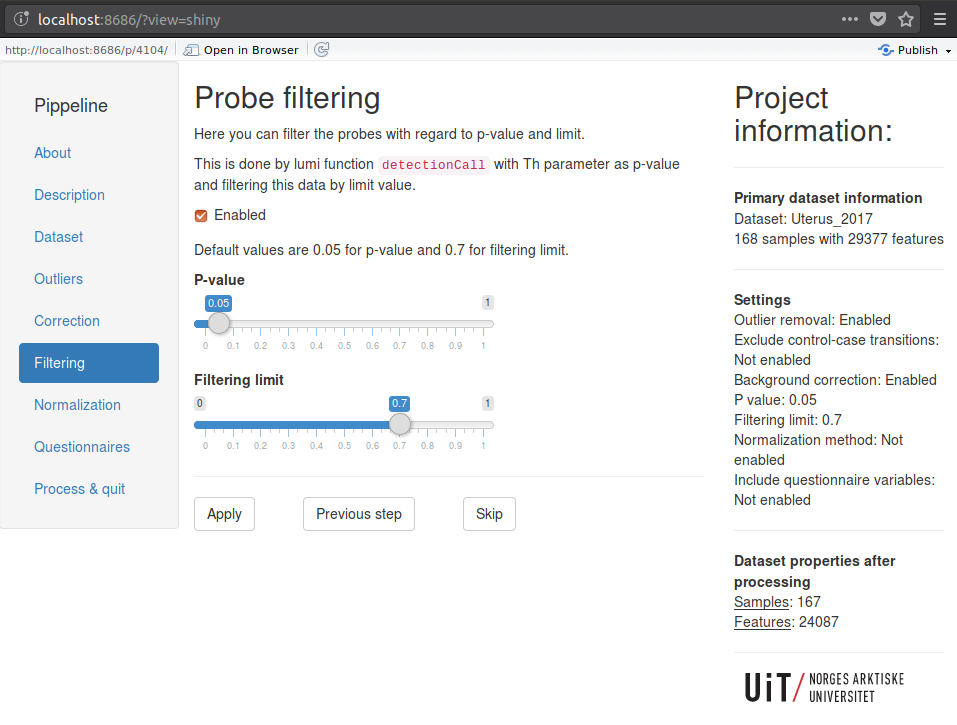
\includegraphics[width=\linewidth]{figures/scr_filtering.png}
  \caption{The Pippeline web application. The screenshot shows the probe
  filtering steps of preparing a gene expression dataset.}
  \label{fig:scr_filtering}
\end{figure}

The Pippeline is implemented as an interactive web application, and users click
through a series of steps before receiving an analysis-ready datasets. 
Users specify details such as what type of study design, e.g. cross-sectional or
case-control, the data normalization methods, and integration with the
questionnaires. 

The Pippeline is implemented as an interactive web application written in R
using the \texttt{Shiny} framework.  Besides the \texttt{shiny} framework, the
Pippeline uses several handful packages for the data analysis, such as
\texttt{lumi}, \texttt{limma}, \texttt{sva}, \texttt{genefilter}, \texttt{nlme}
and \texttt{Biobase}. These packages provide tools for managing our datasets,
methods for processing and analysis. 


% \section{Analysis Pipelines}
% Watchdog:
% https://bmcbioinformatics.biomedcentral.com/articles/10.1186/s12859-018-2107-4
% maybe this one
% http://gopherdata.io/post/more_go_based_workflow_tools_in_bioinformatics/

% \section{Interactive Applications} 
